\documentclass[a4paper,twoside,master.tex]{subfiles}
\begin{document}
\lecture{21}{Monday, March 02, 2020}{Non-Ideal Systems}

\begin{equation}
    H = \sum_{i=1}^{N} \frac{\va{p}_i^2}{2m} + \sum_{i<j} \Phi(\abs{\va{r}_i - \va{r}_j})
\end{equation}

Typically, this potential goes to infinity as $ r \to 0 $, but tends to act attractively as $ - \frac{1}{r^6} $ farther away. Between this attraction and repulsion, there's a minimum where particles can bind and interact. The extra repulsion should make the pressure bigger, while the extra attraction should make the pressure smaller, although the winner will probably be determined by the temperature.

We can write the entropy as
\begin{equation}
    S(U,V,N) = k_B\ln{\int \frac{\dd[3N]{p} \dd[3N]{q}}{h^{3N} N!} \delta(U-H(\{q,p\}))}
\end{equation}
Why don't we just figure out what this is? We can't actually do this integral in any nice way. However, we have an empirical way out. We can make an educated guess for how the free energy changes (in comparison to an ideal gas). For an ideal gas, we can calculate the free energy as

\begin{equation}
    F_{\text{ideal}}(T,V,N) = -N k_B T \left[ \frac{3}{2} \ln\left( k_B T \right) + \ln\left( \frac{V}{N} \right) + X \right]
\end{equation}

Van der Waals' inspired modification to this:
\begin{equation}
    F(T,V,N) = - N k_B T \left[ \frac{3}{2} \ln\left( k_BT \right) + \ln\left( \frac{V\color{red}-Nb\color{black}}{N} + X \right) \right] \color{red}- a \frac{N^2}{V}\color{black}
\end{equation}
where $ a $ and $ b $ are free parameters. Van der Waals' did this for his PhD thesis (no pressure), but why? 

\begin{itemize}
    \item When he decided to replace $ V \to V-Nb $, he figured he should reduce the total accessible volume, since volume is taken up by the gas particles themselves.
    \item The first $ N $ in $ - a \frac{N^2}{V} = N \left[ -a \frac{N}{V} \right] $ keeps the equation extensive. The minus sign refers to a reduction in free energy due to an attraction between nearby particles, and that attraction is proportional to the density $ \frac{N}{V} $.
\end{itemize}

\begin{figure}[h]
    \centering
    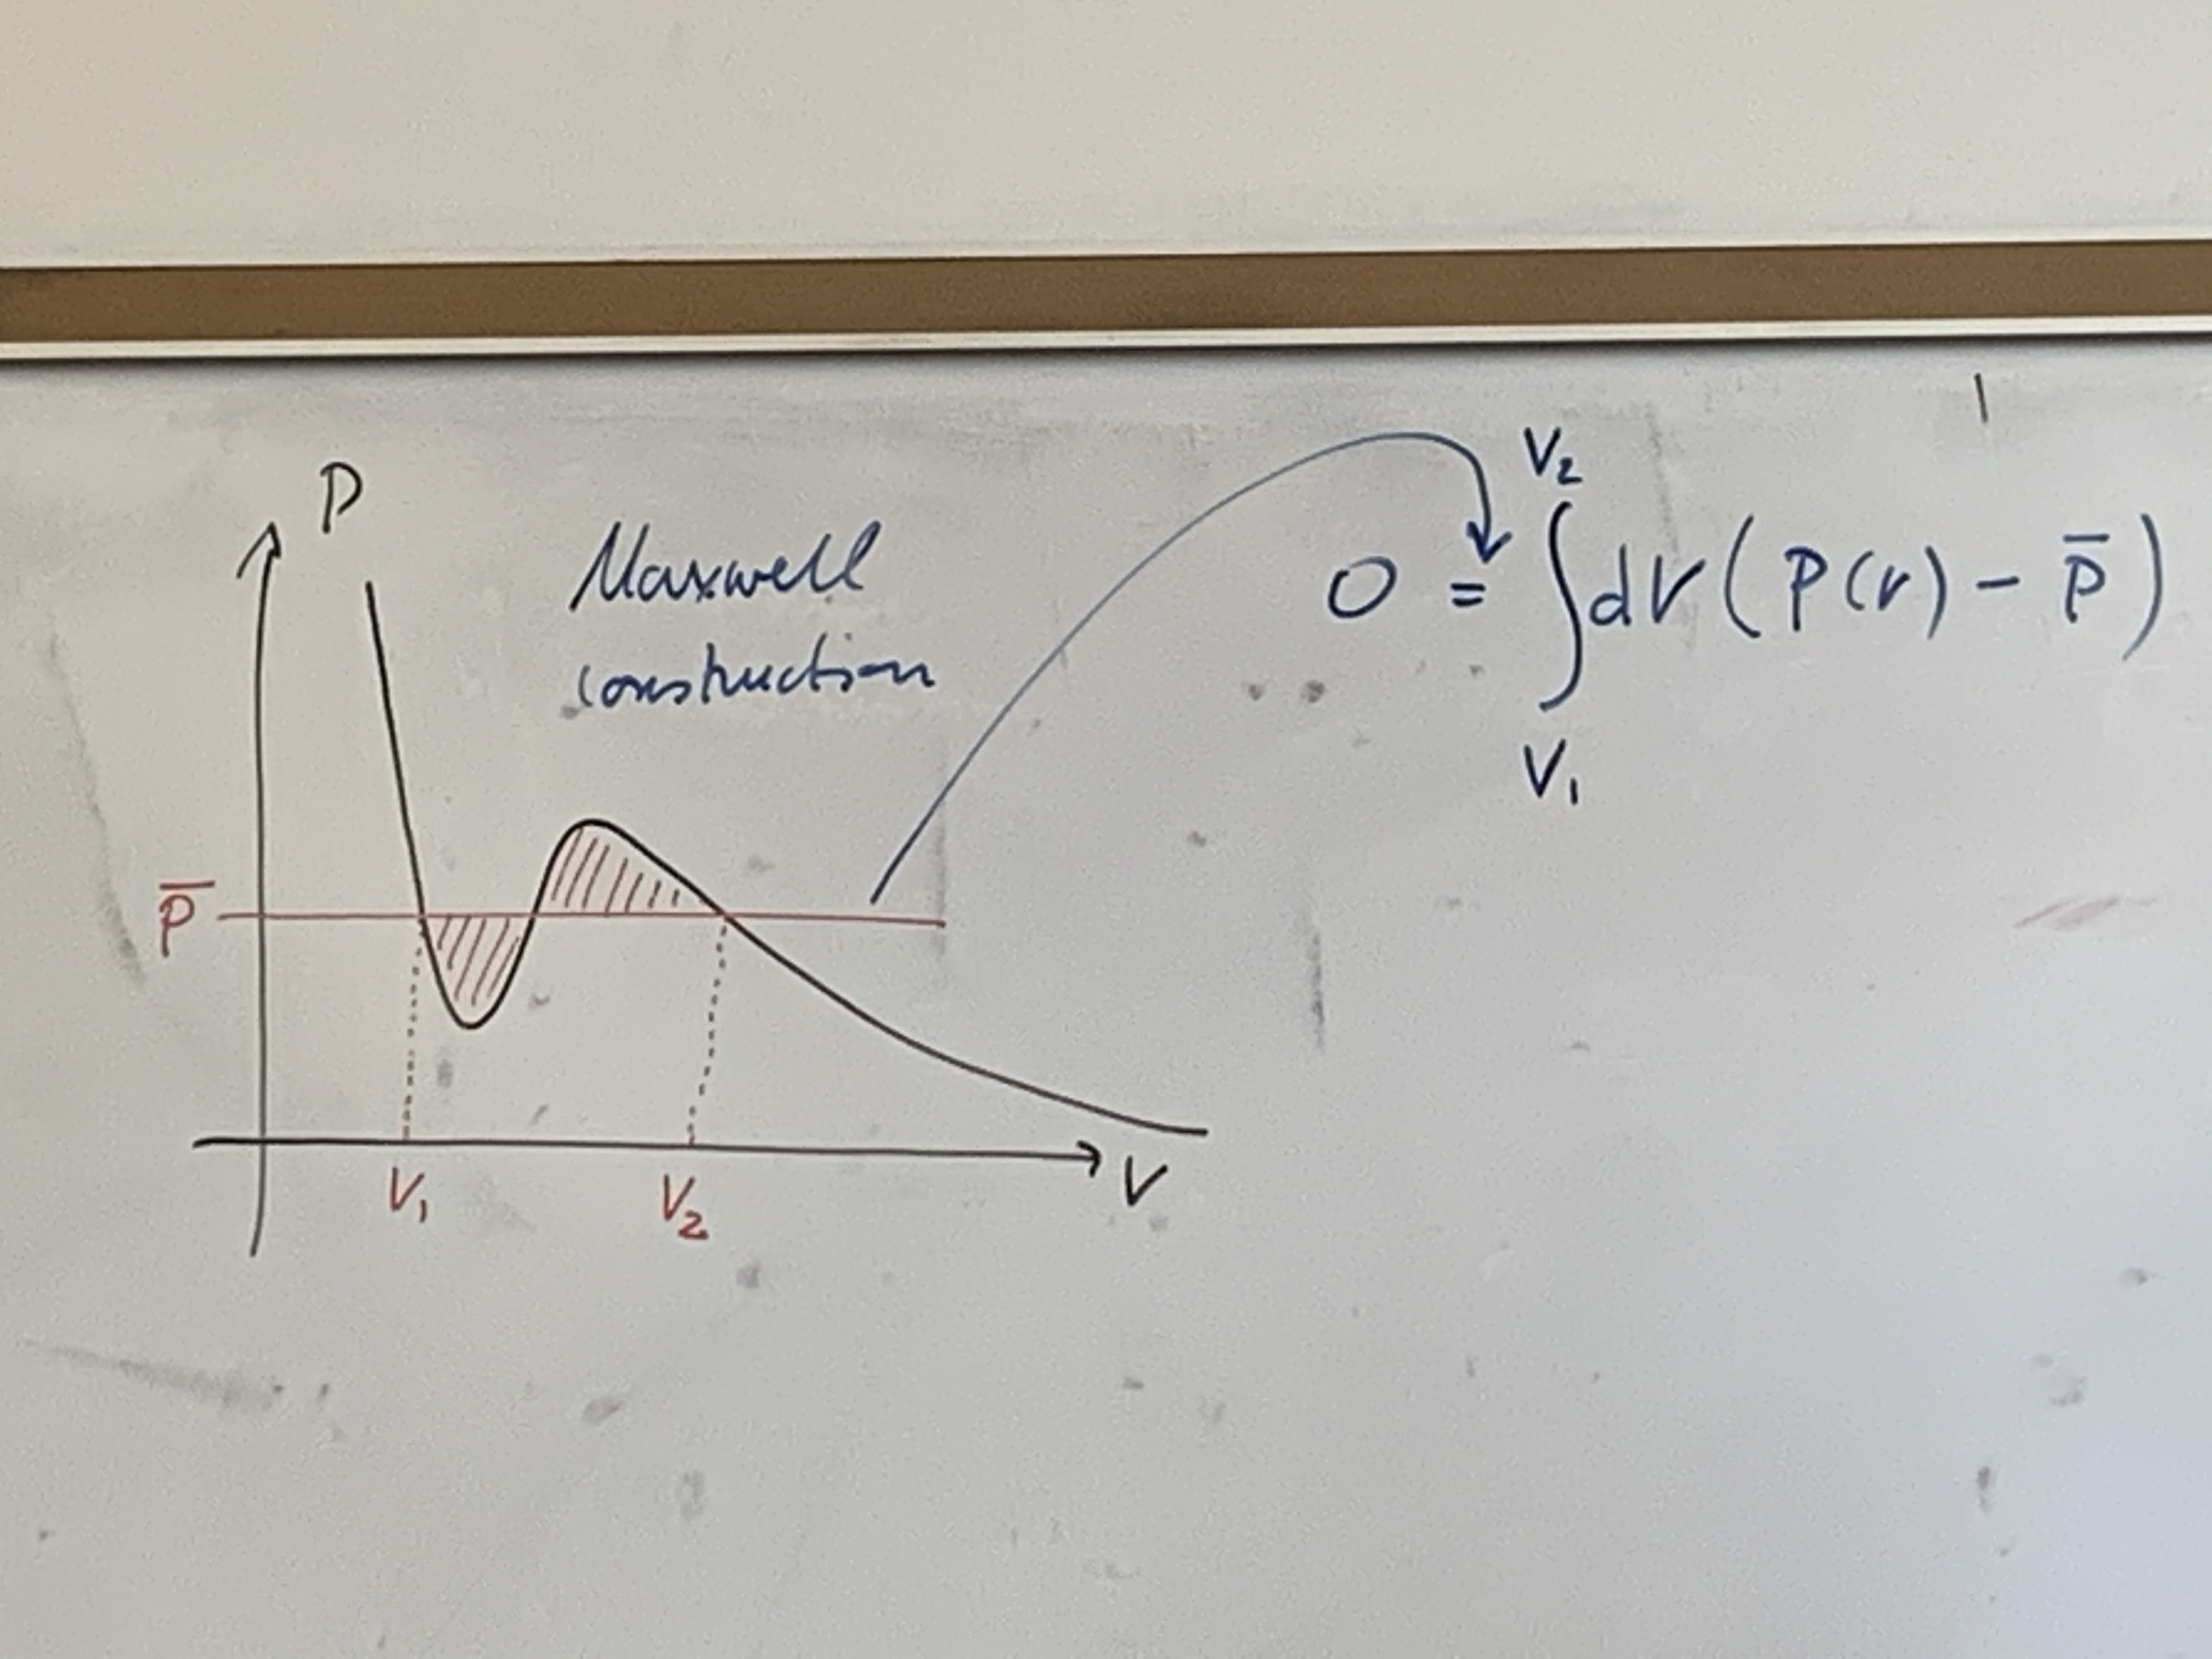
\includegraphics[width=\textwidth]{figures/lec_21_maxwell.png}
    \caption{Diagram of the Maxwell Construction}
    \label{fig:lec_21_maxwell}
\end{figure}

This free energy has some interesting consequences. If we plot pressure-volume curves, we see that there is a region of temperature for which the curve is not convex (as it should be). In particular, there is a pressure $ \bar{P} $ for which the area under the curve is equal to the area above the curve (see \Cref{fig:lec_21_maxwell}). This is called a Maxwell construction. We can write this as
\begin{equation}
    0 = \int_{V_1}^{V_2} \dd{V} \left( P(V) - \bar{P} \right) = \int_{V_1}^{V_2} \dd{V} \left( - \pdv{F}{V} - \bar{P} \right) = - \left( F(V_2) - F(V_1) \right) - \bar{P} \left( V_2 - V_1 \right)
\end{equation}
so
\begin{equation}
    \bar{P} = - \frac{F(V_2) - F(V_1)}{V_2 - V_1} = - F'(V_2) = - F'(V_1)
\end{equation}
This term is the slope of the line connecting $ (V_1, F(V_1)) $ with $ (V_2, F(V_2)) $. The fact that this is equal to the slopes of the tangents of $ F $ at $ V_1 $ and $ V_2 $ is interesting. This line is called a double tangent to $ F $ (see \Cref{fig:lec_21_convex_envelope}).

\begin{figure}[h]
    \centering
    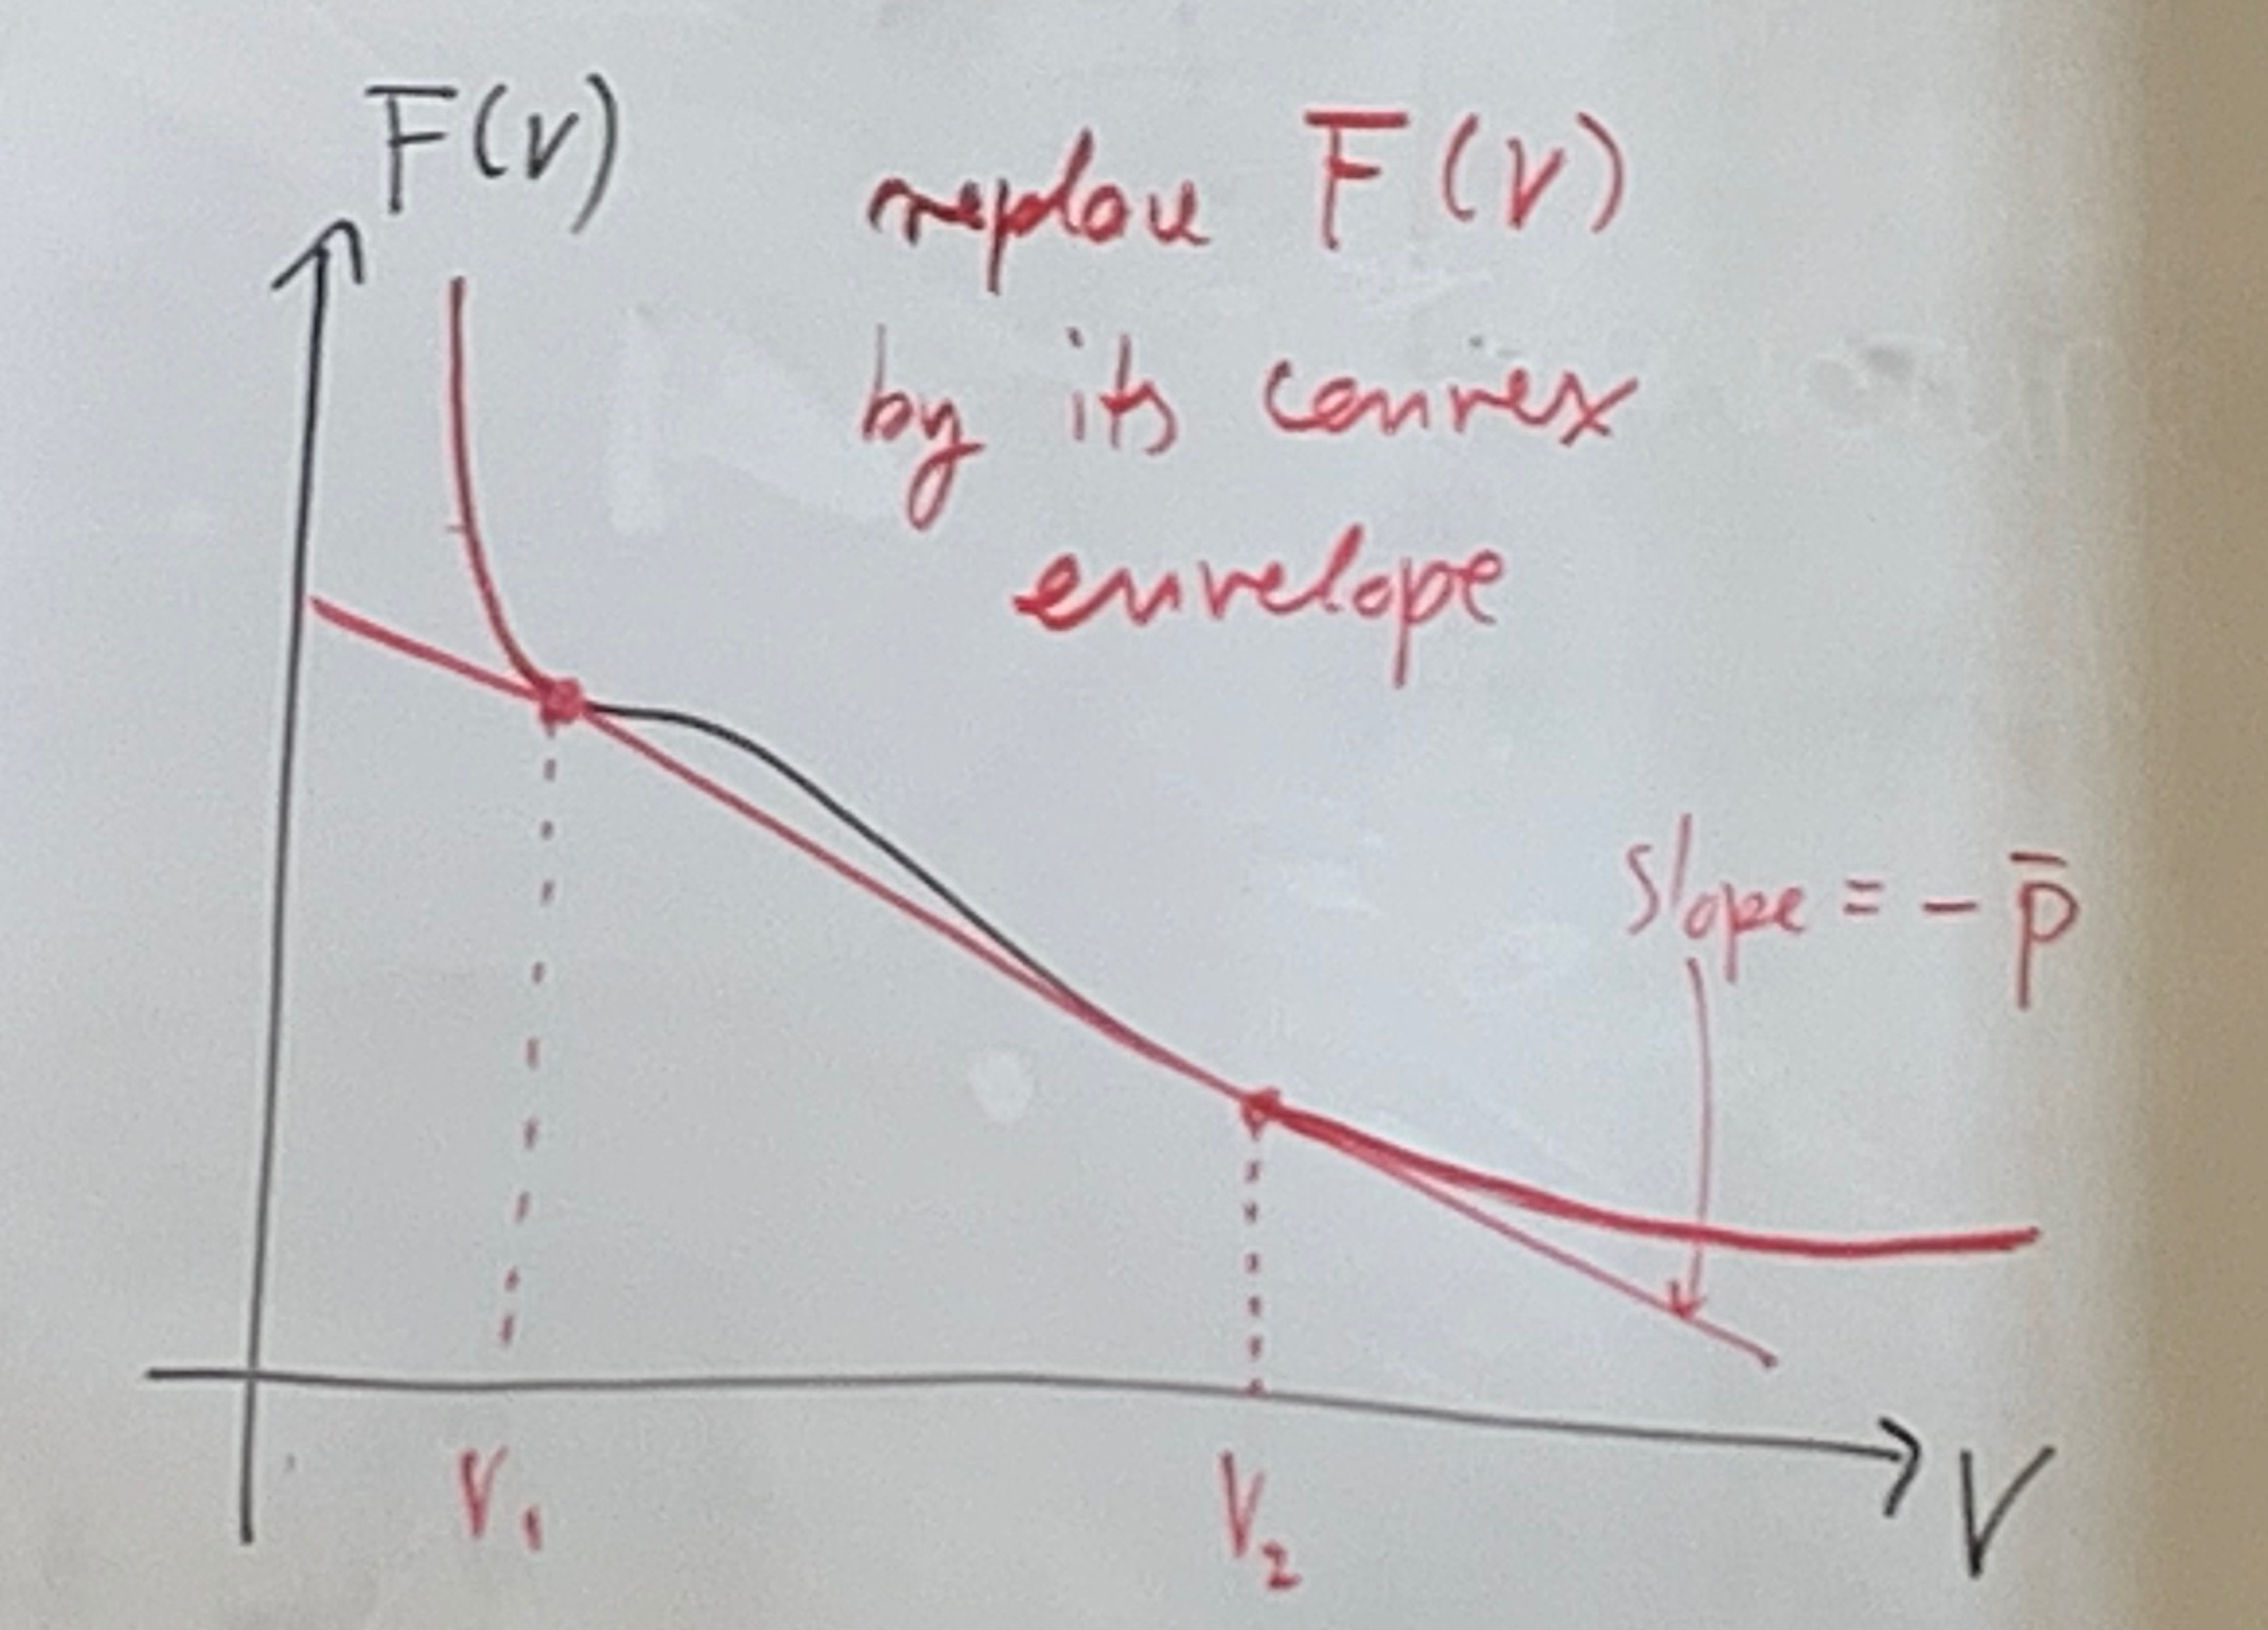
\includegraphics[width=\textwidth]{figures/lec_21_convex_envelope.png}
    \caption{The double tangent line forms a convex envelope of the free energy}
    \label{fig:lec_21_convex_envelope}
\end{figure}

In the next lecture, we will discuss why this is the correct construction.

\end{document}
